\documentclass[12pt]{article}

\usepackage[margin=1in]{geometry}
\usepackage{amsmath,amsthm,amssymb,amsfonts,graphicx}

\newcommand{\Pp}{\emph{\emph{P}}}

\begin{document}

\title{Statistics Homework 4}
\author{Mr. Grant}
\maketitle

\textbf{Due Date:} Tuesday, July 18th \\

Turn in this homework:
\begin{itemize}
	\item On a sheet of lined notebook paper
	\item With your name, the date, and the name of this class on it
	\item With each problem clearly numbered
	\item With your work shown
\end{itemize}

\begin{enumerate}
	\item The mean of Aaliyah, Branden, Carter, and Daniel's shoe sizes is 9. Aaliyah is a size 8, Branden a size 11, and Carter a size 6.5. What is Daniel's shoe size?
	\item There are 5 students in a sample: Ephraim, Felicia, Giselle, Harry, and Ingrid. Ephraim owns 8 pairs of shoes, Felicia owns 20, Giselle owns 30, and Harry owns 3. Suppose you are told that the median number of shoes owned in this sample is 8. What is the largest number of shoes that Ingrid could own? The smallest? Now suppose you are told that the median is 20. What is the largest number of shoes that Ingrid could own? The smallest?
	\item In the group Jasmine, Kyungmin, Leticia, Mokoa, and Naira, Jasmine and Mokoa each have 1 sibling and Kyungmin and Leticia have 2. You are told that the mode of this group is 1. How many siblings does Naira have?
	\item Draw a histogram of the shoe sizes of the Texans in the class, using bins of width 1.
	\item The image below is called a ``frequency histogram"; rather than the number of US households in each column, it shows the percentage of US households in each column. Your friend from Vietnam is visiting the United States for the first time, and you want to help her understand our economy by telling her what a ``typical'' US household earns in a year. Would you tell her the mean household income, the median income (as this graph does), or the mode? Why? (There is no right answer to this question, so what really matters is your explanation.)
\end{enumerate}
\centering
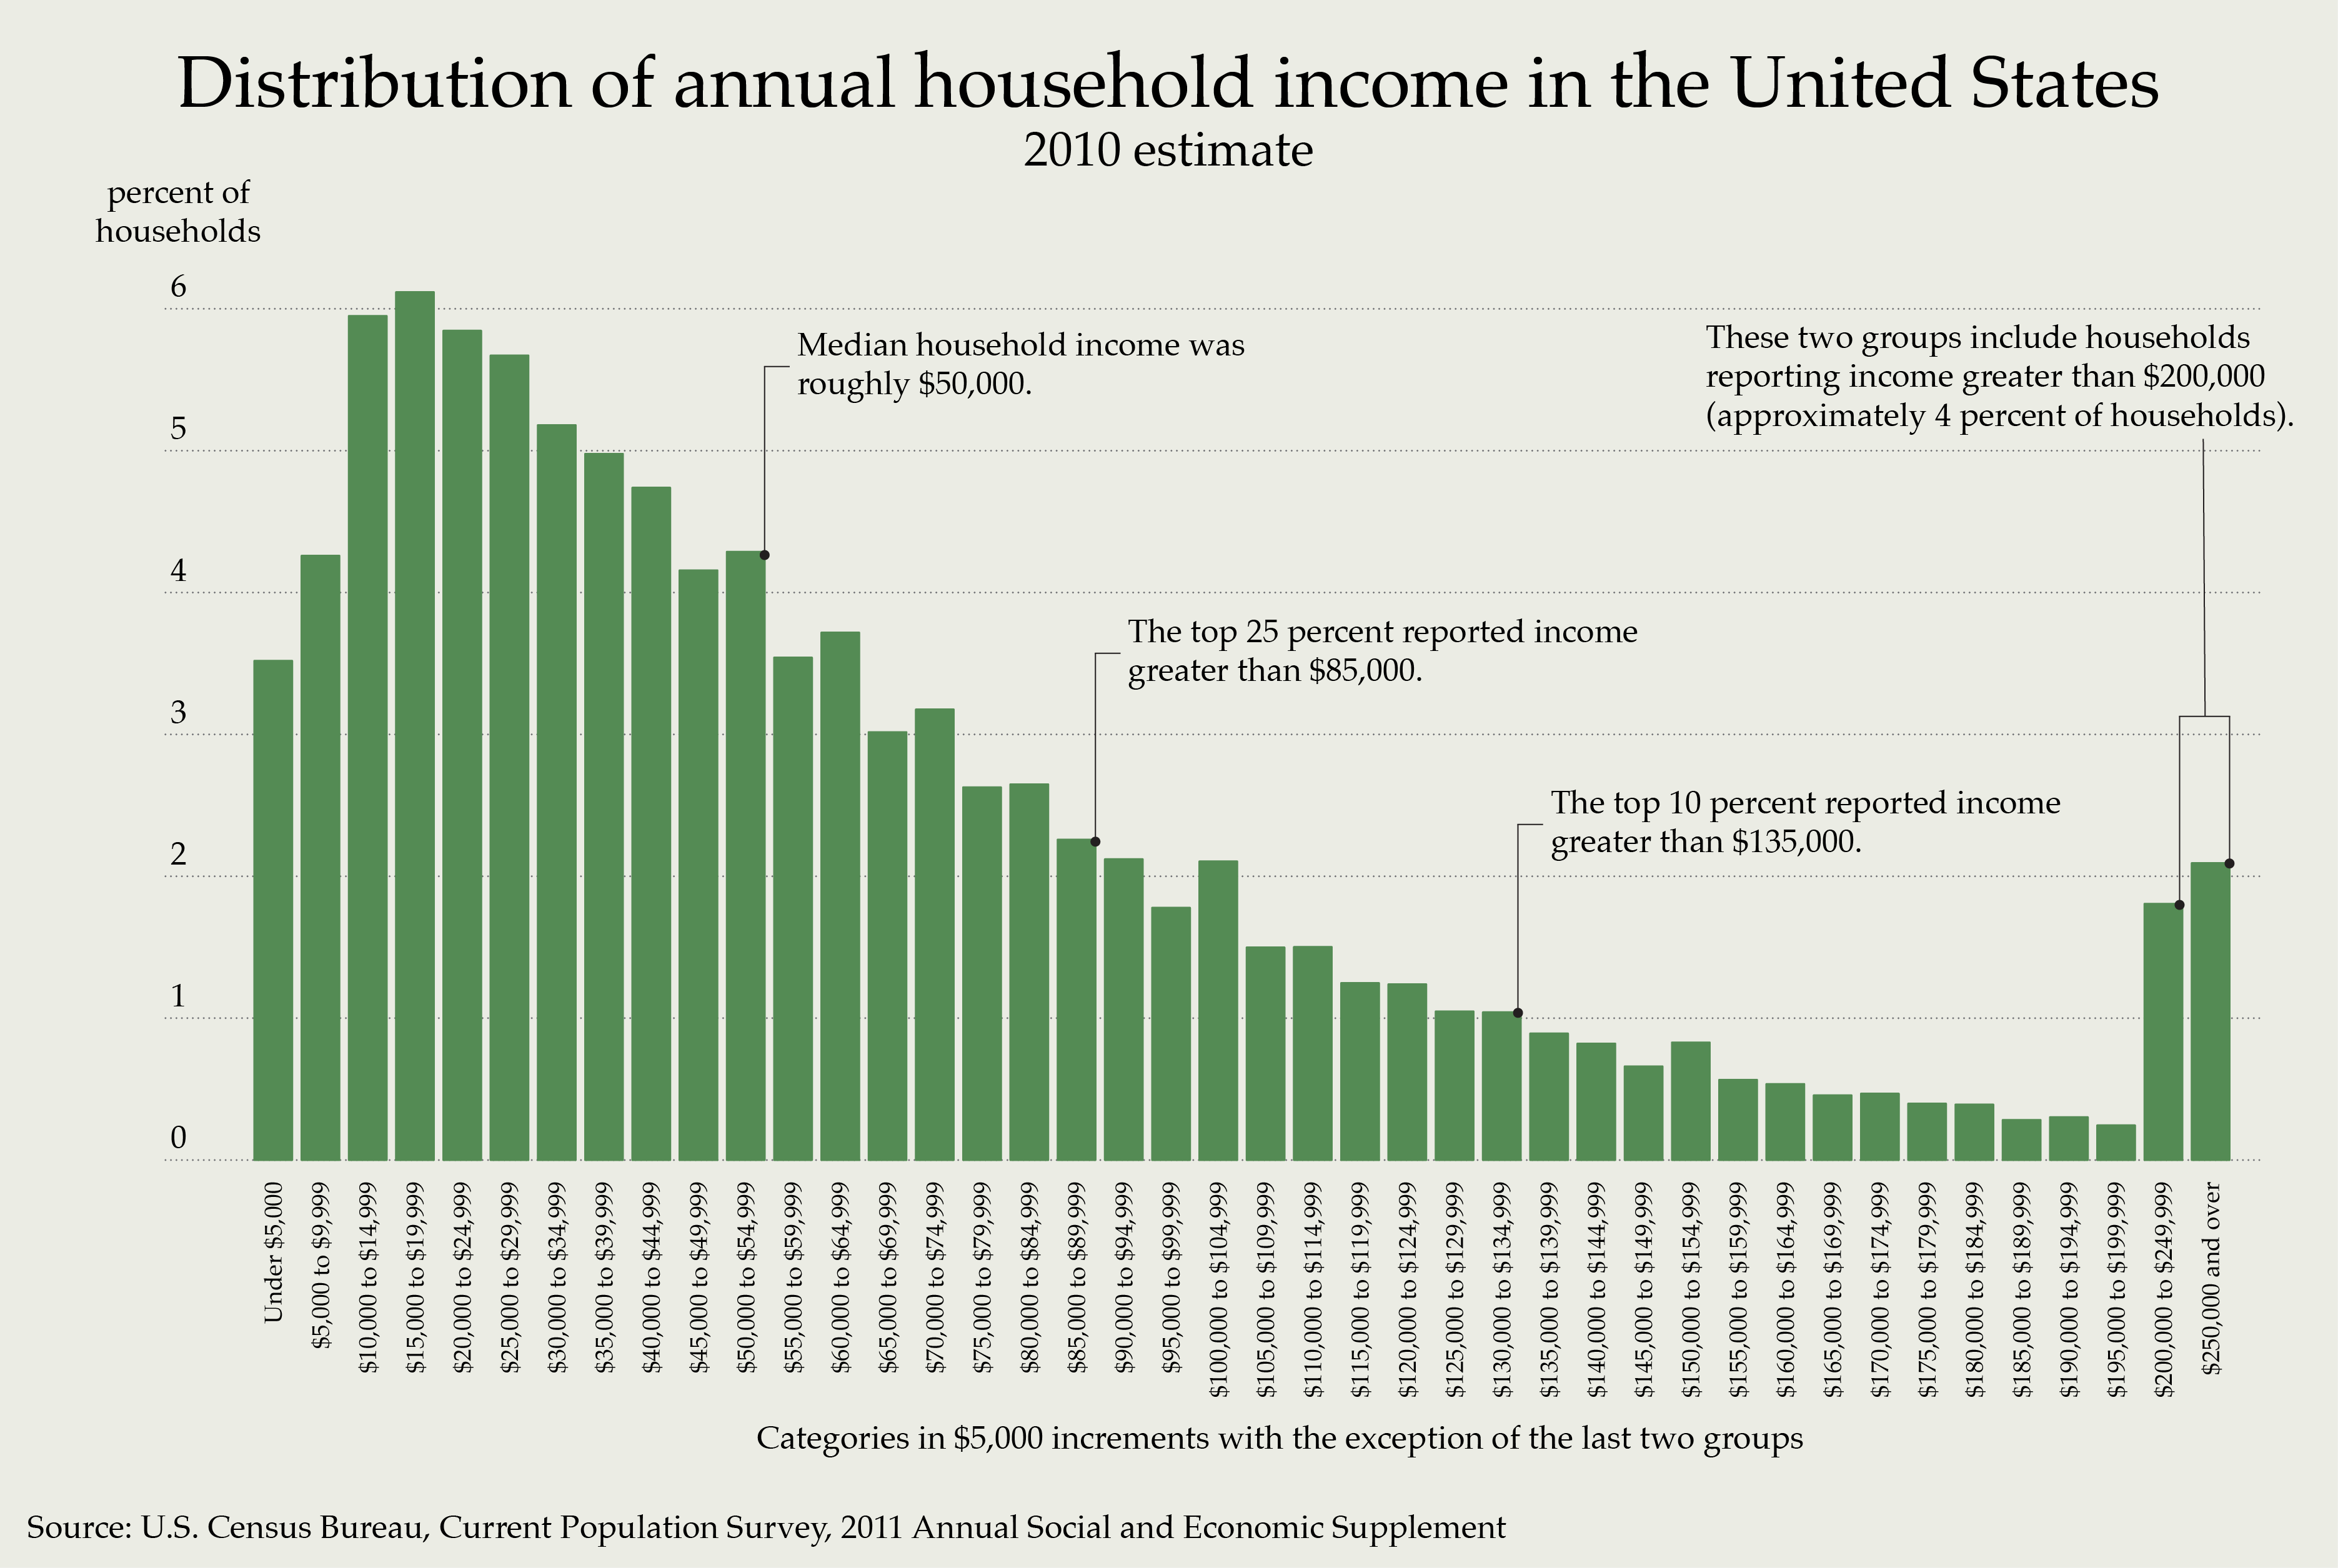
\includegraphics[scale=0.5]{income}
\end{document}
